\documentclass[preprint,12pt]{article}

\usepackage{algorithmic}
\usepackage{algorithm}
\usepackage{enumerate}
\usepackage{enumitem}
\usepackage{graphics}
\usepackage{graphicx}
\usepackage{geometry}
\usepackage{amsmath}
\usepackage{wrapfig}
\usepackage{subfig}
\usepackage{framed}
\usepackage{color}
\usepackage{bm}

\usepackage{multirow}
\usepackage[T1]{fontenc}
\usepackage[latin9]{inputenc}
%\usepackage{units}
\usepackage{esint}

\geometry{legalpaper,  margin=1in}
%\makeatother

%\usepackage{babel}fs

\begin{document}

\section{Modeling the Likelihood of Bias in Future Elections\label{sec:FB}}
 
In order to show that the result is durable -- in other words, that future elections are likely to be impacted, we must, by definition, compute the probabilities of future outcomes given the historical data.  In other words, there are no "actual" results for future harm, since the future hasn't happened yet.  So we can only predict the likelihood of different degrees of harm based on knowledge about the stochastic process and its statistical moments.
 
Our first task in doing this correctly is to select the proper "probability model".  Since we know the underlying process (people voting), we can deduce the correct model from first principles.  In particular, we look at what the underlying Stochastic process is, and how the information that we are interested in relates to it.
 
\subsection{Model selection}
 
Small partisan asymmetries may be observed by chance on an otherwise fairly drawn map. A probability model will allow us to distinguish between cases where an asymmetric result occurred by chance on a fair map, and cases where the legislative map was drawn such that asymmetry is a persistent feature. 
 
To chose a model appropriately, we must carefully consider the underlying process. The Beta distribution is a natural choice for many processes that involve percentages, and is appropriate for modeling election outcomes. This choice of probability model for modeling an election is not new. It has been used in numerous academic papers, and continues to be used in literature published quite recently. ( Paolino 2001, Kaplan and Barnett 2002, Murr 2015)  Indeed, teaching materials about the Beta distribution often use elections as an example.  Some academic papers have extended this model to take into account third parties by using the Dirichlet distribution (Rigdon et al 2009).  (The Dirichlet distribution is the multivariate extension of the Beta distribution.) 
 
The choice of the Beta distribution follows directly from first principles. In fact, two different points of view of the underlying stochastic process of election results both lead us to the Beta distribution. In our present case, depending on our point of view, the underlying stochastic process is either a Bernoulli process (a number of trials that can each have one of two outcomes -- votes that can be for either one party or another) or a pair of Poisson processes (a series of events occurring at a certain rate -- voters for a party turning out to cast a vote).  
 
In the first perspective (Bernoulli process), we are interested in the number of votes for a given party out of all the votes - the number of "successes" in a sequence of trials.  This leads us to the Binomial distribution.  However, we do not know the rate of "successes" - that is what we are trying to estimate.  To estimate the rate parameter of a Binomial distribution, we use its "conjugate prior distribution", which is the Beta distribution.
 
In the second perspective (Poisson process), we are interested in the number of times a voter for a party turns out to vote in a given amount of time (Election day) - the number of events in a fixed interval. This leads us to the Poisson distribution.  However, we do not know the rate of "events" - that is what we are trying to estimate.  To estimate the rate parameter of a Poisson distribution, we use its "conjugate prior distribution", which is the Gamma distribution.  However, we are not done yet - we are interested in what fraction of events between the two poisson processes are from the first.  Where G(X) is the (unknown) rate of voter turnout for one party, and G(Y) the (unknown) rate for the other, we are interested in G(X) / ( G(X) + G(Y) ).  This leads us to the Beta distribution.
 
Thus, deduction from first principles leads us to select the Beta distribution as our probability model for the outcome of an election, regardless of which perspective we initially take.
 
\subsection{Parameter estimation}
 
Now that we have selected the appropriate probability distribution (Beta), the next task is to estimate the parameters of the distribution.  Since we are estimating the parameters of a "prior" distribution -- that is, we are using a Beta distribution to model the distribution of the parameter p of a Binomial distribution -- directly from empirical data, what we are doing is called an "Empirical Bayes method".
 
Ideally, we'd use the maximum likelihood method for estimating the parameters, but unfortunately the Beta distribution does not have a closed form solution for that, so instead we use the method-of-moments .  We estimate the parameters of the Beta distribution of the total popular vote, and for the popular vote in each district.  
 
To estimate the second moment (variance), we use an unbiased estimator.  The primary difference is that the statistical dispersion is a little greater.  Because we use an unbiased estimator, our model is also a model of future elections, not just previous elections.  More precisely, using an unbiased estimator makes our model a model of the "population" as opposed to only the "samples".
 
Note that to construct a seats-votes curve, we need to mean-center the total votes before estimating the parameters for the districts.  This has the added benefit that it helps to take into account systemic correlations among the districts.  That is, it encapsulates any information about uniform partisan swings in the likelihood function for the statewide vote totals, and removes this extra variance from the district totals.

A summary of this probability model is shown in figure \ref{fig:ProbabilityModel}.

\begin{figure}[htb!]
    \begin{center}
        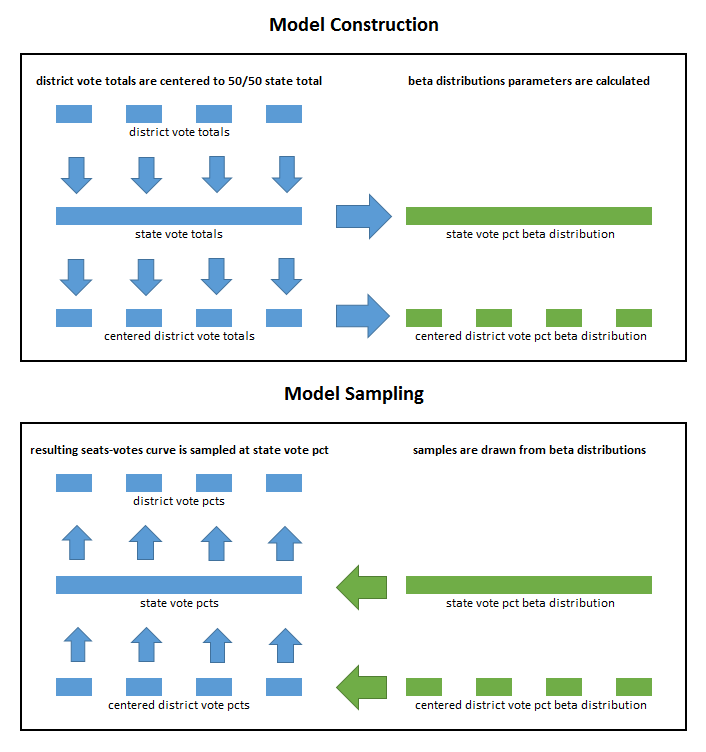
\includegraphics[scale=1.0]{../Figures/WI2010/probabilityModel.png}
        \caption{Probability model for future election outcomes}\label{fig:ProbabilityModel}
    \end{center}
\end{figure}

Shown in figure \ref{fig:SVCongress} are twelve sample seats-votes curves and popular vote percentages drawn from such a probability model, using the 2012, 2014, and 2016 Wisconsin congressional election vote counts as inputs.  The solid curve is the seats-votes curve.  The dashed curve is the 2-axis reflection of the seats-votes curve.  The dotted vertical line is the popular vote percentage.  The drawn samples show a consistent and large asymmetry in favor of Republicans.

\begin{figure}[htb!]
    \begin{center}
        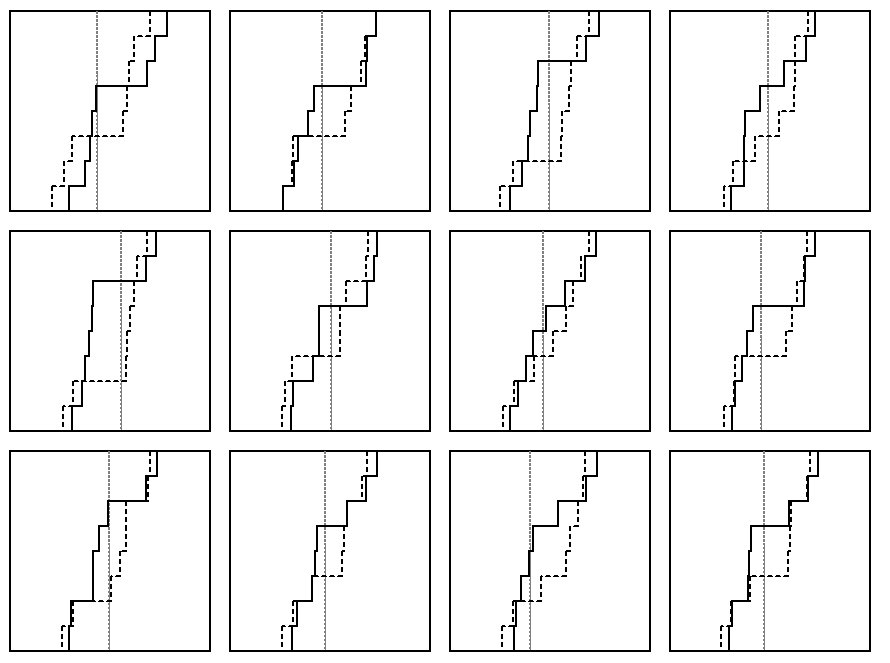
\includegraphics[scale=0.6]{../Figures/WI2010/sv_curves_congress.png}
        \caption{Some election outcome seats-votes curves generated from the probability model}\label{fig:SVCongress}
    \end{center}
\end{figure}
 
\subsection{Extending the model with the Gamma distribution}
 
The basic model outlined above does not give vote counts, only vote percentages.  To extend the model to one that estimates vote counts, one can use Gamma distribution to model voter turnout, both at the district level and at the state level.
 
First we estimate the statewide Gamma distributions, as well as the average statewide turnout over all sample elections.   Then we take the district counts for each election and multiply them by a per-election constant factor to make their statewide totals match the average statewide totals.  Then we estimate the per-district Gamma parameters from those average-centered numbers.
 
To draw an outcome from this hierarchical model, we first draw vote percentages from the basic model. Then we draw turnouts from the average-centered per-district Gamma distributions, then we use the drawn per-district vote percentages to split those into the Democratic turnout and Republican turnout.  We do the same with the statewide turnout -- we draw a sample and split it into Democratic and Republican vote turnout. 
 
Finally, for each party, we multiply the per-party-per-district turnout by a constant factor to match the per-party-statewide turnout.  This gives us vote counts for each party and district, whose vote percentages match the basic model, and whose turnouts match the turnout model.
 
As a sanity check, we compared results of the extended model with the basic model.  Our tests showed that the two models are in very strong agreement. 
 
 
\subsection{Using empirical priors for 1-sample tests or to improve estimates}
 
This method of creating a probability model is good when you have enough historical elections to create a model from, but what if you have data for only 1 election?
 
If you have only 1 historical election, you can use your single sample as the mean of the Beta distribution, and for the variance of the Beta distribution you can use the expectation of the historical variance since 1972.
 
We computed the standard deviation (unbiased estimate) for the 2 party democratic vote share over the redistricting cycle for federal congressional elections from 1972-2016 for all states in the country. We ignored uncontested elections since, with 2,076 data points, we had plenty of data to compute a typical standard deviation from without the need to impute missing data.
 
Shown in figure \ref{fig:Hyperprior} is a histogram of the results.  The mean is 6.1\%, the median is 5.2\%, and close to 85\% of districts had a standard deviation of less than 10\%. 

\begin{figure}[htb!]
    \begin{center}
        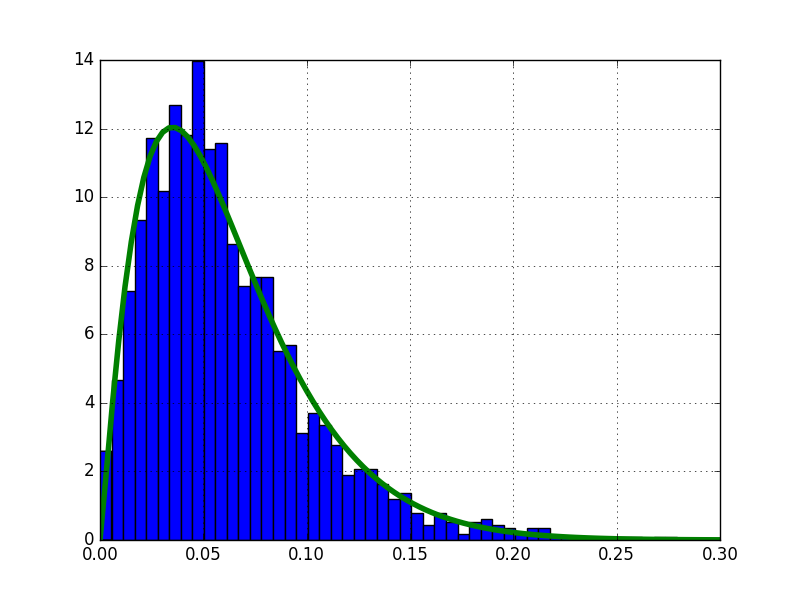
\includegraphics[scale=0.6]{../Figures/WI2010/hyperprior.png}
        \caption{Hperprior of district partisianship standard deviation}\label{fig:Hyperprior}
    \end{center}
\end{figure}
 
For a single sample, one can use the expectation of the standard deviation -- 6.1\% or 0.061 -- as a plug-in estimator for the standard deviation. (The variance is the square of this: 0.003721.)  Then one can combine that with their single sample serving as the mean, and use the method of moments to estimate the alpha and beta parameters of the Beta distribution for each district.
 
For more than 1 sample, to improve the accuracy of an estimator, one can fit the histogram to a Beta distribution (since the values vary between 0 and 1).  We computed the alpha and beta parameters of a fitted Beta distribution (shown by the green line in the chart) using maximum likelihood estimation (MLE). They come out to:
 
\{ alpha: 2.17183630081, beta: 33.2358219613 \}
 
You can use this Beta distribution as a Bayesian prior on the standard deviation for district partisanship for federal congressional elections.  Then you can compute the maximum likelihood estimation of the Beta distribution parameters for each district by way of Bayes' Rule.  
 
That is, where p(A) is the prior likelihood of having a given standard deviation according to the above graph, and p(B|A) is the conditional probability of the observations (B) given the standard deviation A and the sample mean, the most likely standard deviation given the data p(A|B) is the one that maximizes the likelihood of p(B|A)*p(A): 

Additionally we could go a step deeper and, instead of calculating the expected value of p(A|B), integrate over all possible values for A, weighted by their posterior likelihoods, p(A|B).

\subsection{Comparison to tests for asymmetry in the statistics literature}
 
Numerous tests have been proposed to determine if a given set of data is likely to be asymmetric, see (Zheng and Gastwirth 2010, Mira 1999, Cabilio and Masaro 1996) and the references therein. These tests are based on the well understood and widely used concepts of statistical hypothesis testing. An example of the hypothesis testing approach applied to gerrymandering is the mean median difference test proposed by Dr. Sam Wang, a neuroscience professor from Princeton University (Wang 2016). While some parallels exist between the procedure employed here and these tests, there are some crucial differences. Speaking broadly, we may contrast the hypothesis testing approach with the proposed approach in the following terms. For the statistical hypothesis testing approach, one must assume an underlying symmetric model for the data that is regarded as a suitable benchmark, and determine how likely it is for this reference model to produce an asymmetry at least as large as that observed in the actual election data. In contrast, the proposed procedure constructs a model from the data as they actually are, allowing one to evaluate the tendency of a map to produce asymmetric results. 
 
Using statistical hypothesis testing for assessing asymmetry in a legislative map attempts to answer the following question: if we assume that a map is fair, then how likely is it for us to observe an asymmetry at least as large as the asymmetry of an actual election? If the probability of observing an asymmetry at least as extreme as the one encountered in an actual result (the so called p-value of the test) is less than a certain threshold, often 5\%, the we can claim with a high degree of certainty that the electoral results are not symmetric. In such a framework, small deviations from asymmetry will be allowed, since we could not say whether or not such deviations occurred by chance with much certainty. On the other hand, large deviations which can not be expected to occur by chance would not be allowed.
 
There are two important aspects of statistical tests for asymmetry that are evident from the literature, which are summarized most succinctly in (Zheng and Gastwirth 2010). First, the choice of the so called null distribution, or the underlying symmetric model that is used as a benchmark for determining which deviations from symmetry may be the result of chance, has an effect on the results of the test. Standards based on one particular null distribution (the unit normal distribution is the most common) may be more or less permissive in detecting asymmetry. The literature also shows that it is prudent to use numerical integration to find the p-value of the test, since while p-values can be computed from formulas without integration, these are applicable for large sample sizes and may lead to errors for states with fewer than 20 or so districts. 
 
In spite of this, the statistical hypothesis testing approach remains a valid and extremely useful methodology for examining and diagnosing gerrymandering. In fact, since the statistical models used as a benchmark for comparison for such tests assume that each district has the same probability distribution for it's voting percentages (i.e. the districts are assumed independent and identically distributed), the hypothesis testing approach will tend to be more permissive than the approach described here. In particular, gerrymanders that are small in magnitude but highly durable may slip through the cracks. 
 
Voter's preferences tend to be stable, and bias in electoral maps also are very stable particularly if they are large, as shown by the expert witness testimony in Whitford v Gil. Given this information, one could assume that an observed bias is likely to be a persistent feature of an electoral map. Alternatively, the model described here could be used to directly assess the likelihood of persistent bias in a map on a case by case basis since it makes use of additional information that is not employed in the statistical hypothesis testing approach. Namely, districts need not be assumed to be identically distributed, but rather each district is modeled with it's own distribution that reflects the preferences of its constituency. As described in section C, the process of voting may be modeled with well known probability distributions and using these gives us a model that possesses a level of detail not achievable using the statistical hypothesis testing approach.
 
With either approach we can not avoid specifying a probability model and further we should use numerical integration to ensure the most accurate possible results. The difference between the two approaches therefore boils down to what the probability models represent, as well as the details of those models themselves. With the hypothesis testing approach, we compare a reference symmetric probability model with the actual election results. With the current approach, we create a probability model from the election results and determine how likely the model is to produce asymmetric results. Since voting preferences and bias in electoral maps historically are very stable, the statistical hypothesis testing approach is a powerful method for examining gerrymandering that is simple and conventional. The current approach allows one to examine the bias in an electoral map in greater detail, providing valuable insight on the persistence of bias in the map. Both approaches are in close agreement for the Wisconsin state assembly, identifying a large and durable gerrymander in favor of Republicans.
 
\section{Numerical Integration of Likelihoods}
 
The partisan asymmetry likelihood function can be generated by integrating the statewide and district partisanship likelihood functions.  As these distributions, like most Bayesian models, don't lend themselves to analytic integration, numerical integration must be used. Since our model involves multiple integration and a random process, we use the Monte-Carlo numerical integration method.
 
We draw a sample from both the statewide popular vote distribution, and the individual district vote distribution.   From the individual district distributions, we construct a seats-votes curve.  We then sample the seats votes curve at the point we drew from the popular vote distribution, and at its inverse - 1 minus that, giving us both the number of seats Republicans would get at that vote fraction, and the number of seats Democrats would get if the vote fraction was reversed.  We then take the simple difference of the two, and "bin" it.  We repeat this process 100,000 times.  This takes a couple of seconds on a typical desktop computer.  The result is a well-defined specific partisan asymmetry likelihood curve, from which we can extract very accurate descriptive statistics about not only how gerrymandered a map is, but how durable that gerrymander is.

\subsection{Calculating the partisan asymmetry of a single election}
 
SCOTUS has ruled that seats proportional to votes can not be a legal standard (Thornburg v. Gingles 1986).   But they remain open to a legal standard based on the idea of partisan symmetry.
 
The concept of partisan symmetry is that if a party gets say, 60\% of the seats when they get 55\% of the votes, then a different party should also get 60\% of the seats when they get 55\% of the votes.  This is a somewhat looser criteria than saying that the seats must be proportional to the votes - which simply isn't possible in a mixture of winner-take-all elections.  But it still retains the notion of equality of speech, which is the key principle behind democracy, and enshrined in the "one person, one vote" principle of Baker v. Carr.  Violating partisan symmetry means that people's right to representation were abridged because of their political beliefs.
 
To measure deviation from that ideal, we construct a curve of all possible vote percentages and their corresponding results.  This can be constructed easily and quickly from the by-district vote counts.

\begin{enumerate}

\item First, we mean-center all the votes.
\begin{enumerate}
\item First, compute the total counts for each party
\item Then take the average of that over all parties
\item Then take the votes in each district for each party, divide by the total across the state for that party (from step a), and multiply by the average (from step b).
\end{enumerate}
\item Then we sort the districts from most Democratic to most Republican

\end{enumerate}

Let's say that the district with the highest percentage of Democratic partisanship has 70\% Democratic votes and 30\% Republican (after mean centering), in order for at least 50\% of the votes to be Republican, we must apply a state-wide swing of 30\%-70\%.  That'll make that district exactly 50\%-50\%, and all of the other districts majority Republican.  So at 30\% Democratic vote we have exactly 1 Democratic seat, any lower and we have 0.
 
Whenever the vote percentage hits the inverse (1-x) of the vote percentage of one of the mean-centered districts, that district turns from not won by that party to won by that party.  And we can count this up and get number of seats from number of votes.   So we have our seats-votes curve.
 
Notice also that this recapitulates all of the information we have about the partisanship of the districts.   Indeed, it is simply the partisanship of the districts, mean centered so that the popular vote is 50-50, and then sorted.
 
Below is a picture of the seats-votes curve for Wisconsin assembly districts for the 2012 election after imputing uncontested seats with the presidential vote, along with a "symmetry line".  (The average of the curve and its reflection about the origin.)  The shaded area represents partisan asymmetry.  This curve is fairly atypical because it shows an unusually high amount of asymmetry.
 
Recall that the curve recapitulates the district vote totals.  Comparing the seats-votes curve with its mirror image shows how lopsided the partisan composition of the districts are.  The fact that in the lower right, the seats-votes curve is to the left of symmetry, shows that democratic districts are packed more than republican districts. Similarly, the bulge in the middle shows that republican districts are cracked more than democratic districts.

 
\subsection{"Specific" partisan asymmetry}
 
To calculate partisan asymmetry at a given popular vote percentage, you simply find out how many seats one party would obtain at that vote percentage, and subtract how many seats the other party would get if they got that same percentage of popular votes.  Now that we have the seats-votes curve, we can look that up easily.
 
By "specific" partisan asymmetry, we mean the partisan asymmetry at the popular vote percentage that actually occurred in the given election.   The advantage of "specific" partisan asymmetry is that it gives, not just a measure of potential harm to citizens, but a measure of actual harm that has already been done to citizens with a particular political preference.
 
We can add this value up over multiple elections, to get the cumulative harm done over the course of the redistricting cycle.
 
Since the measure is in terms of difference in congressional seats, we can count the number of citizens harmed by simply multiplying the difference in congressional seats by the average population of a district.  This gives us both the effective number of artificially "added" ballots, and the number of artificially "removed" ballots.  Put otherwise, it gives us the number of citizens that were effectively disenfranchised because of their political preference, and the number of citizens that effectively got their vote coutned twice because of their political preference.
  
\subsection{Advantages of this metric}
 
Before applying this metric to a concrete example, we'd like to highlight some of the advantages of this metric.

\begin{itemize}

\item Doesn't assume proportionality in results - The seats-votes curve for single-winner elections naturally take on a cumulative Beta-binomial distribution, as opposed to a diagonal line representing seats proportional to votes.  This metric doesn't assume a diagonal curve representing proportionality.  It tests a looser (less strict) criteria: asymmetry, which still retains the essential feature of measuring disenfranchisement based on political belief.  SCOTUS has ruled that seats proportional to votes can not be a legal standard (Thornburg v. Gingles 1986).   But they remain open to a legal standard based on the idea of partisan symmetry.
 
\item Distinguishes between artificial partisan bias and the natural multiplying effect of single-winner elections -  Single-winner aka "Majoritarian" elections naturally over-favor the majority party, giving them a larger fraction of the seats than they get of the popular vote.  While some measures might mistakenly identify this as gerrymandering, specific asymmetry explicitly takes this into account by calculating and then subtracting this natural multiplying effect.
 
\item Works for states with partisanship far from 50/50 - By sampling the asymmetry at the actual vote counts rather than e.g. 50/50, this metric maintains full relevance even for the most extremely partisan states.
 
\item Takes into account non-uniform swings - By looking at not only the average partisanship of each district, but how much the partisanship of each individual district changes from election to election, this metric is able to take into account the changes in voter sentiment that are not uniform throughout the state; that are perhaps concentrated in only certain districts.

\item Shows durability - By computing an entire likelihood function for specific partisan asymmetry, rather than a single point estimate, this metric enables quick and accurate assessment of how durable a gerrymander is; how much more harm it will cause in the future, including what the likelihood is that it will not cause harm.
 
\item Measures partisan vote packing - Asymmetry in the seats-votes curve measures imbalance between how one party's voters are packed vs cracked compared to the other's. The specific partisan asymmetry distribution calculates the various likelihoods of that for future elections, using results from actual elections.  Thus, this measure measures, as directly as possible, the unfair advantage given to people with a given political belief (and disadvantage to another) due to partisan vote packing, and the durability of this imbalance.

\item Represents deviation from what is practically achievable - It is trivial for a computer algorithm to design districts that make the seats-votes curve perfectly symmetric, while satisfying all constitutional requirements.  Thus, to convert this absolute score to one relative to what can be accomplished by a redesign that meets all traditional redistricting principles, one simply subtracts zero.  This "new" relative score gives you the number of voters whose votes were effectively stolen by the map drawers with the current map, and whose right to representation can be returned by a remedy map that can be trivially designed by a computer employing a multi-objective heuristic optimization algorithm.

\item It is well-ordered.  It is a monotonic function of actual partisan advantage - Increasing partisan advantage for one party always increases this measure, and vice-versa.  A greater partisan advantage cannot have a lower score, Nor can a higher score represent a lower advantage.  And since we are measuring at actual future outcomes, in proportion to their likelihood, the measure relates monotonically to the actual future partisan advantage.
 
\item The only possible improvements are shift, scale, and shape - Since it is well ordered and monotonic with respect to actual partisan advantage, any "better" measure can only be better in the sense of having a more appropriate "center" point, a more appropriate scale, or a more appropriate "shape" (change of slope as you go up and down the scale).  The scale varies from -1 to 1, which is as ideal as it gets.  The "center",  zero, is a non-arbitrary and very reasonable choice, representing a perfectly symmetric situation.   
 
\item It takes into account all possibilities, weighted by likelihood - Every possible seats-votes curve and every possible popular vote ratio is taken into consideration, weighted by the combined likelihood of the two.
 
\end{itemize}


\section{Partisan Bias in the Wisconsin State Assembly, post 2010 census\label{sec:Wis}}

\subsection{Data preparation}
\subsubsection{Imputing uncontested elections}
 
Some elections are uncontested.   This poses a problem for data analysis, as it amounts to missing data.  There are three ways we can deal with the missing data: 
 

\begin{enumerate}
\item treat them as contested elections with unanimous support, 
\item throw out the uncontested elections, and 
\item estimate what the results would be if they were contested
\end{enumerate}
 
The academic consensus is that the third option leads to the most accurate data analysis.  Indeed, the other two options produce highly skewed results.
 
To estimate the uncontested races, we use the presidential vote count where available, and the federal congressional vote count in years where there was no presidential election.
 
Our imputation process is as follows:
 
\begin{enumerate}
\item Calculate the total votes for each party for both sets of elections, counting only those districts that were contested in both.
\item Multiply the by-district totals in the data set used to impute by the totals in step 1 for the data set with the missing data, and divide by the total in step 1 for the set used to impute.  We call this "swing adjusting", because it makes both data sets have the same overall swing.  It also matches the voter turnout.
\item Substitute in these swing-adjusted districts for the missing data.
\end{enumerate}
 
\subsubsection{De-aggregating and re-aggregating for different precinct shapes (pre-2010 census)}
 
In order to have more data to use, we take imputed data from prior to the post-2010 census maps, de-aggregate them to block level (proportional to voting age population), and then re-aggregate that back to district level, for the post-2010 census districts.
 
We limit the data to only going back a little over 10 years, to keep it recent.  That still gives us 6 elections to work with.
 
\subsection{Future election result likelihoods (District partisanship likelihoods)}
 
Shown in figure \ref{fig:Betas} is a graph of district partisanship, including dispersion.  To generate this graph, a Beta distribution for each district was calculated using the method of moments.  Additionally a Beta distribution for the total popular vote was calculated using the method of moments.  Then the probability density function was plotted out for each one of them.  (The black curve in the middle is the total popular vote.) Results that lead to a Democrat winning the seat are colored in blue, and results that lead to a Republican winning the seat are colored in red.
 
The phenomena of packing and cracking discussed in the above section is clearly evident.  Note, in addition to the the average of the past 6 elections, the graph also shows the statistical dispersion, from which the durability of this effect for future elections can be assessed.

\begin{figure}[htb!]
    \begin{center}
        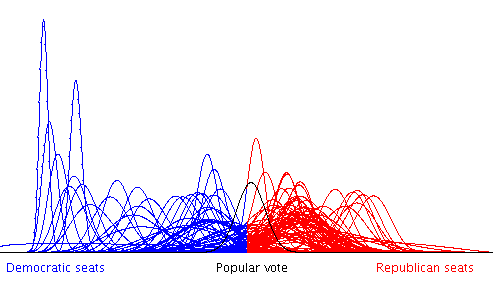
\includegraphics[scale=0.25]{../Figures/WI2010/betas.png}
        \caption{Beta distributions for Wisconsin 2010-cycle Assembly districts}\label{fig:Betas}
    \end{center}
\end{figure}
 
Note that Democratic-leaning districts are both far to the left, showing high partisanship (and thus low voter impact), and low dispersion -- meaning the voters are unlikely to change their minds; they are "safe" Democratic voters.  Conversely, the Republican-leaning districts are closer to the middle, but still safely to the right, and all centered around about the same place.   These are characteristic signs of packing and cracking.  Let me rephrase that: this is the very definition of "packing and cracking".  The Democratic voters were packed - hence far to the left.  By concentrating Democratic voters in few districts, this reduces the number of seats that Democratic voters can win.  The remaining population was "cracked" to get the Republican-leaning districts all to about the same level of moderately (but safely) Republican-leaning partisanship, thus increasing the number of seats that Republican voters can win.  The net effect is to maximize the impact of Republican votes, and minimize the impact of Democratic votes.
 
Shown in figure \ref{fig:SVAssembly} are twelve seats-votes curves drawn from these distributions (solid curve), along with their 2-axis reflection (dashed curve), and a popular vote percentage drawn from the statewide beta distribution (vertical dotted gray line).  A large and consistent asymmetry in favor of Republicans is immediately evident.

\begin{figure}[htb!]
    \begin{center}
        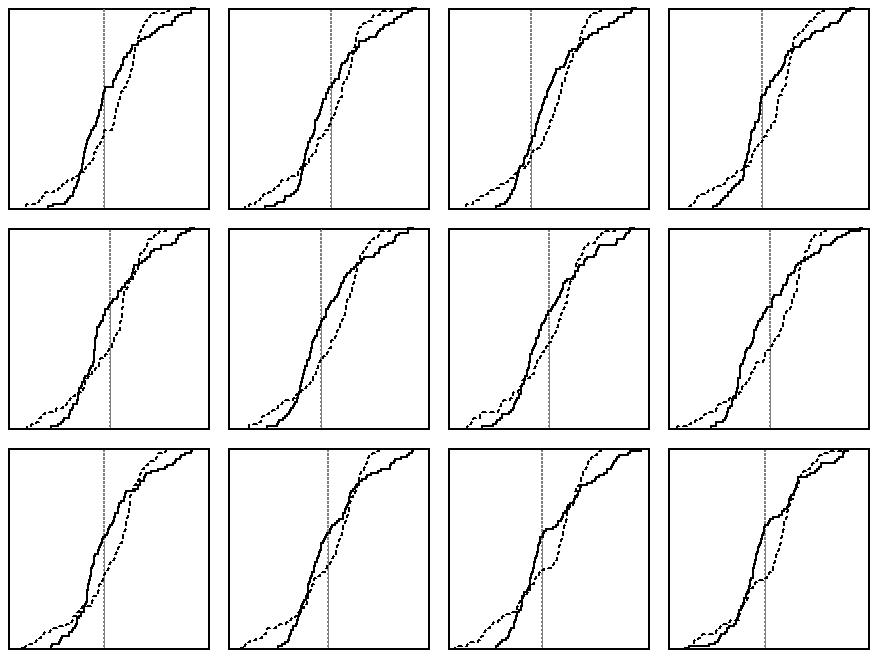
\includegraphics[scale=0.6]{../Figures/WI2010/sv_curves_assembly.png}
        \caption{Some election outcome seats-votes curves generated from the probability model for Wisconsin 2010 Assembly districts}\label{fig:SVAssembly}
    \end{center}
\end{figure}

\subsection{Numerical integrations of likelihood functions}
\subsubsection{District partisanship histogram}
 
Another way we can see this is by looking at the histogram of district partisanship.
 
Similarly to how we modeled vote percentages with Beta distributions, we used Gamma distributions to model voter turnout.  We then combined these two to model actual vote counts in each district.  This allowed us to compute likelihood functions for specific vote counts in every district.  We then used Monte Carlo integration to construct the likelihood function for district partisanship, over all districts.
 
The resulting curve shown in figure \ref{fig:LikelihoodsDistrictPartisanship} leaves no room for interpretation.  The high red peak close to the center but still safely to the side shows that Republican districts are heavily cracked.  Conversely, the mass of blue far to the side and comparative lack of a strong peak close to the center shows that Democratic districts are heavily packed.
 
\begin{figure}[htb!]
    \begin{center}
        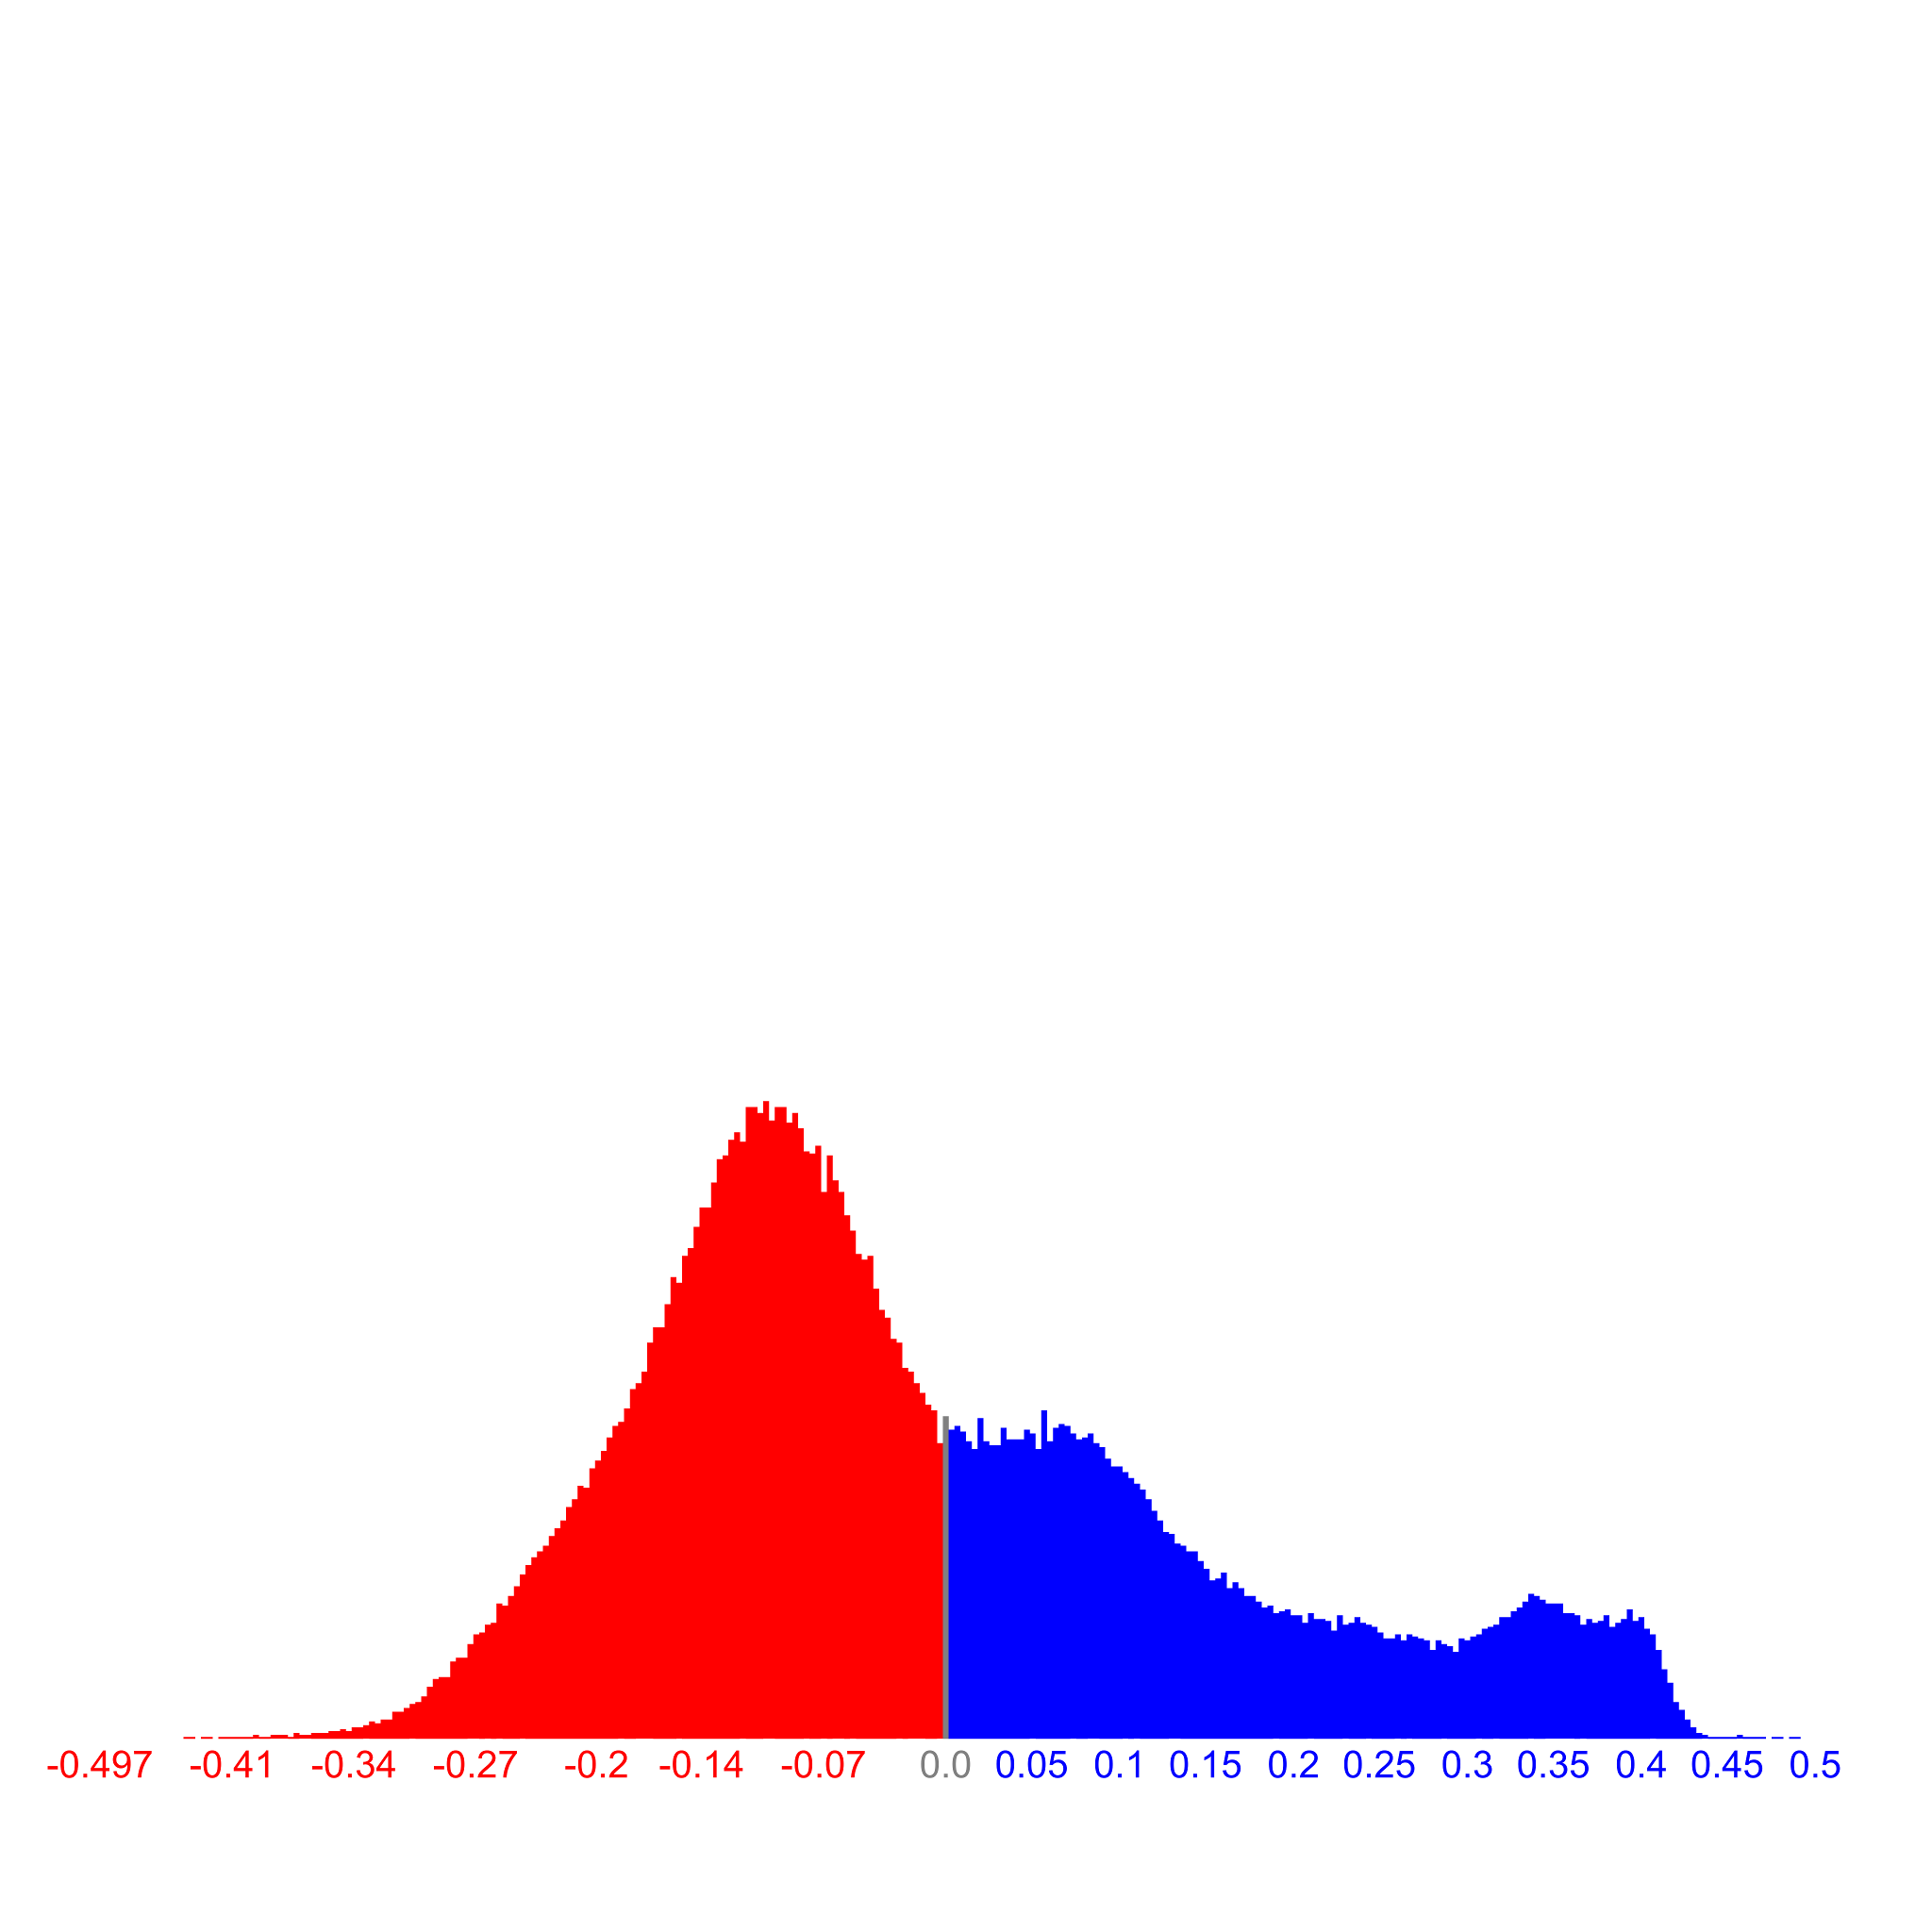
\includegraphics[scale=0.25]{../Figures/WI2010/district_partisanship_new.png}
        \caption{District partisanship likelihoods generated from the probability model for Wisconsin 2010 Assembly districts}\label{fig:LikelihoodsDistrictPartisanship}
    \end{center}
\end{figure}

Comparing this chart with the empirical district partisanship histogram for all U.S. congressional elections for all states since 1972, (figure \ref{fig:LikelihoodsDistrictPartisanshipAll}) we see that it stands in stark congress to the almost even distribution over all cycles, and even stands out from the 2010 cycle, which the Republican State Leadership Committee has openly advertised that they successfully gerrymandered (REDMAP).

\begin{figure}[htb!]
    \begin{center}
        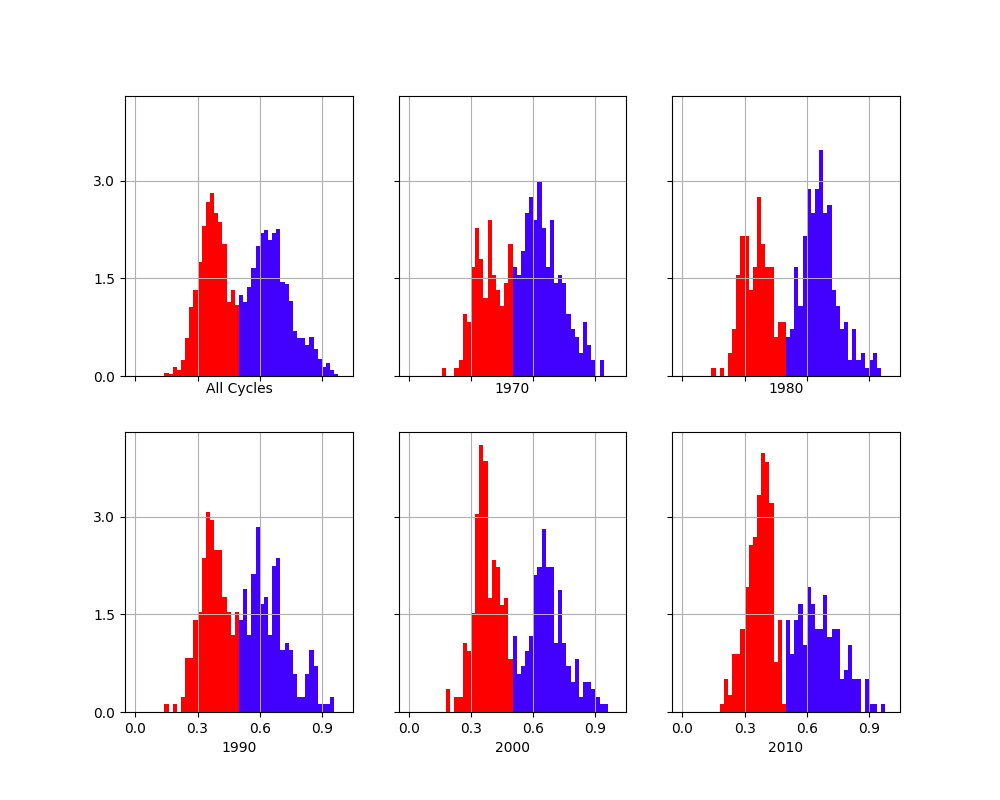
\includegraphics[scale=0.5]{../Figures/WI2010/cycle_partisan_likelihoods.png}
        \caption{Empirical district partisanship likelihoods for all Congressional districts in the United States from 1972 to 2016}\label{fig:LikelihoodsDistrictPartisanshipAll}
    \end{center}
\end{figure}
 
\subsubsection{Statewide seat count likelihoods}
 
The seat count likelihoods produced by this packing and cracking can be shown by integrating the statewide and district partisanship likelihood functions.  As these distributions, like most Bayesian models, don't lend themselves to analytic integration, numerical integration must be used. Using the Monte-Carlo numerical integration method, with 100,000 samples, we constructed the probability mass function for the Republican seat count results from an election, given the current districts and voter demographics.  The results are shown in figure \ref{fig:LikelihoodsSeatCounts}.
 
Particularly striking about this result is that, while the popular vote likelihoods in the above graph centers around 50/50, favoring Democratic representatives more than 40\% of the time, the seat count likelihoods never put Democratic representatives in the majority.  Indeed, out of 100,000 samples, it never even gives them 44 out of 99 of the seats.  On average Republican representatives maintain a 63-36 seat advantage.   This shows a sizable and durable partisan advantage for Republicans, despite the actual voters showing no clear preference, and indeed, preferring Democrats almost half the time.

\begin{figure}[htb!]
    \begin{center}
        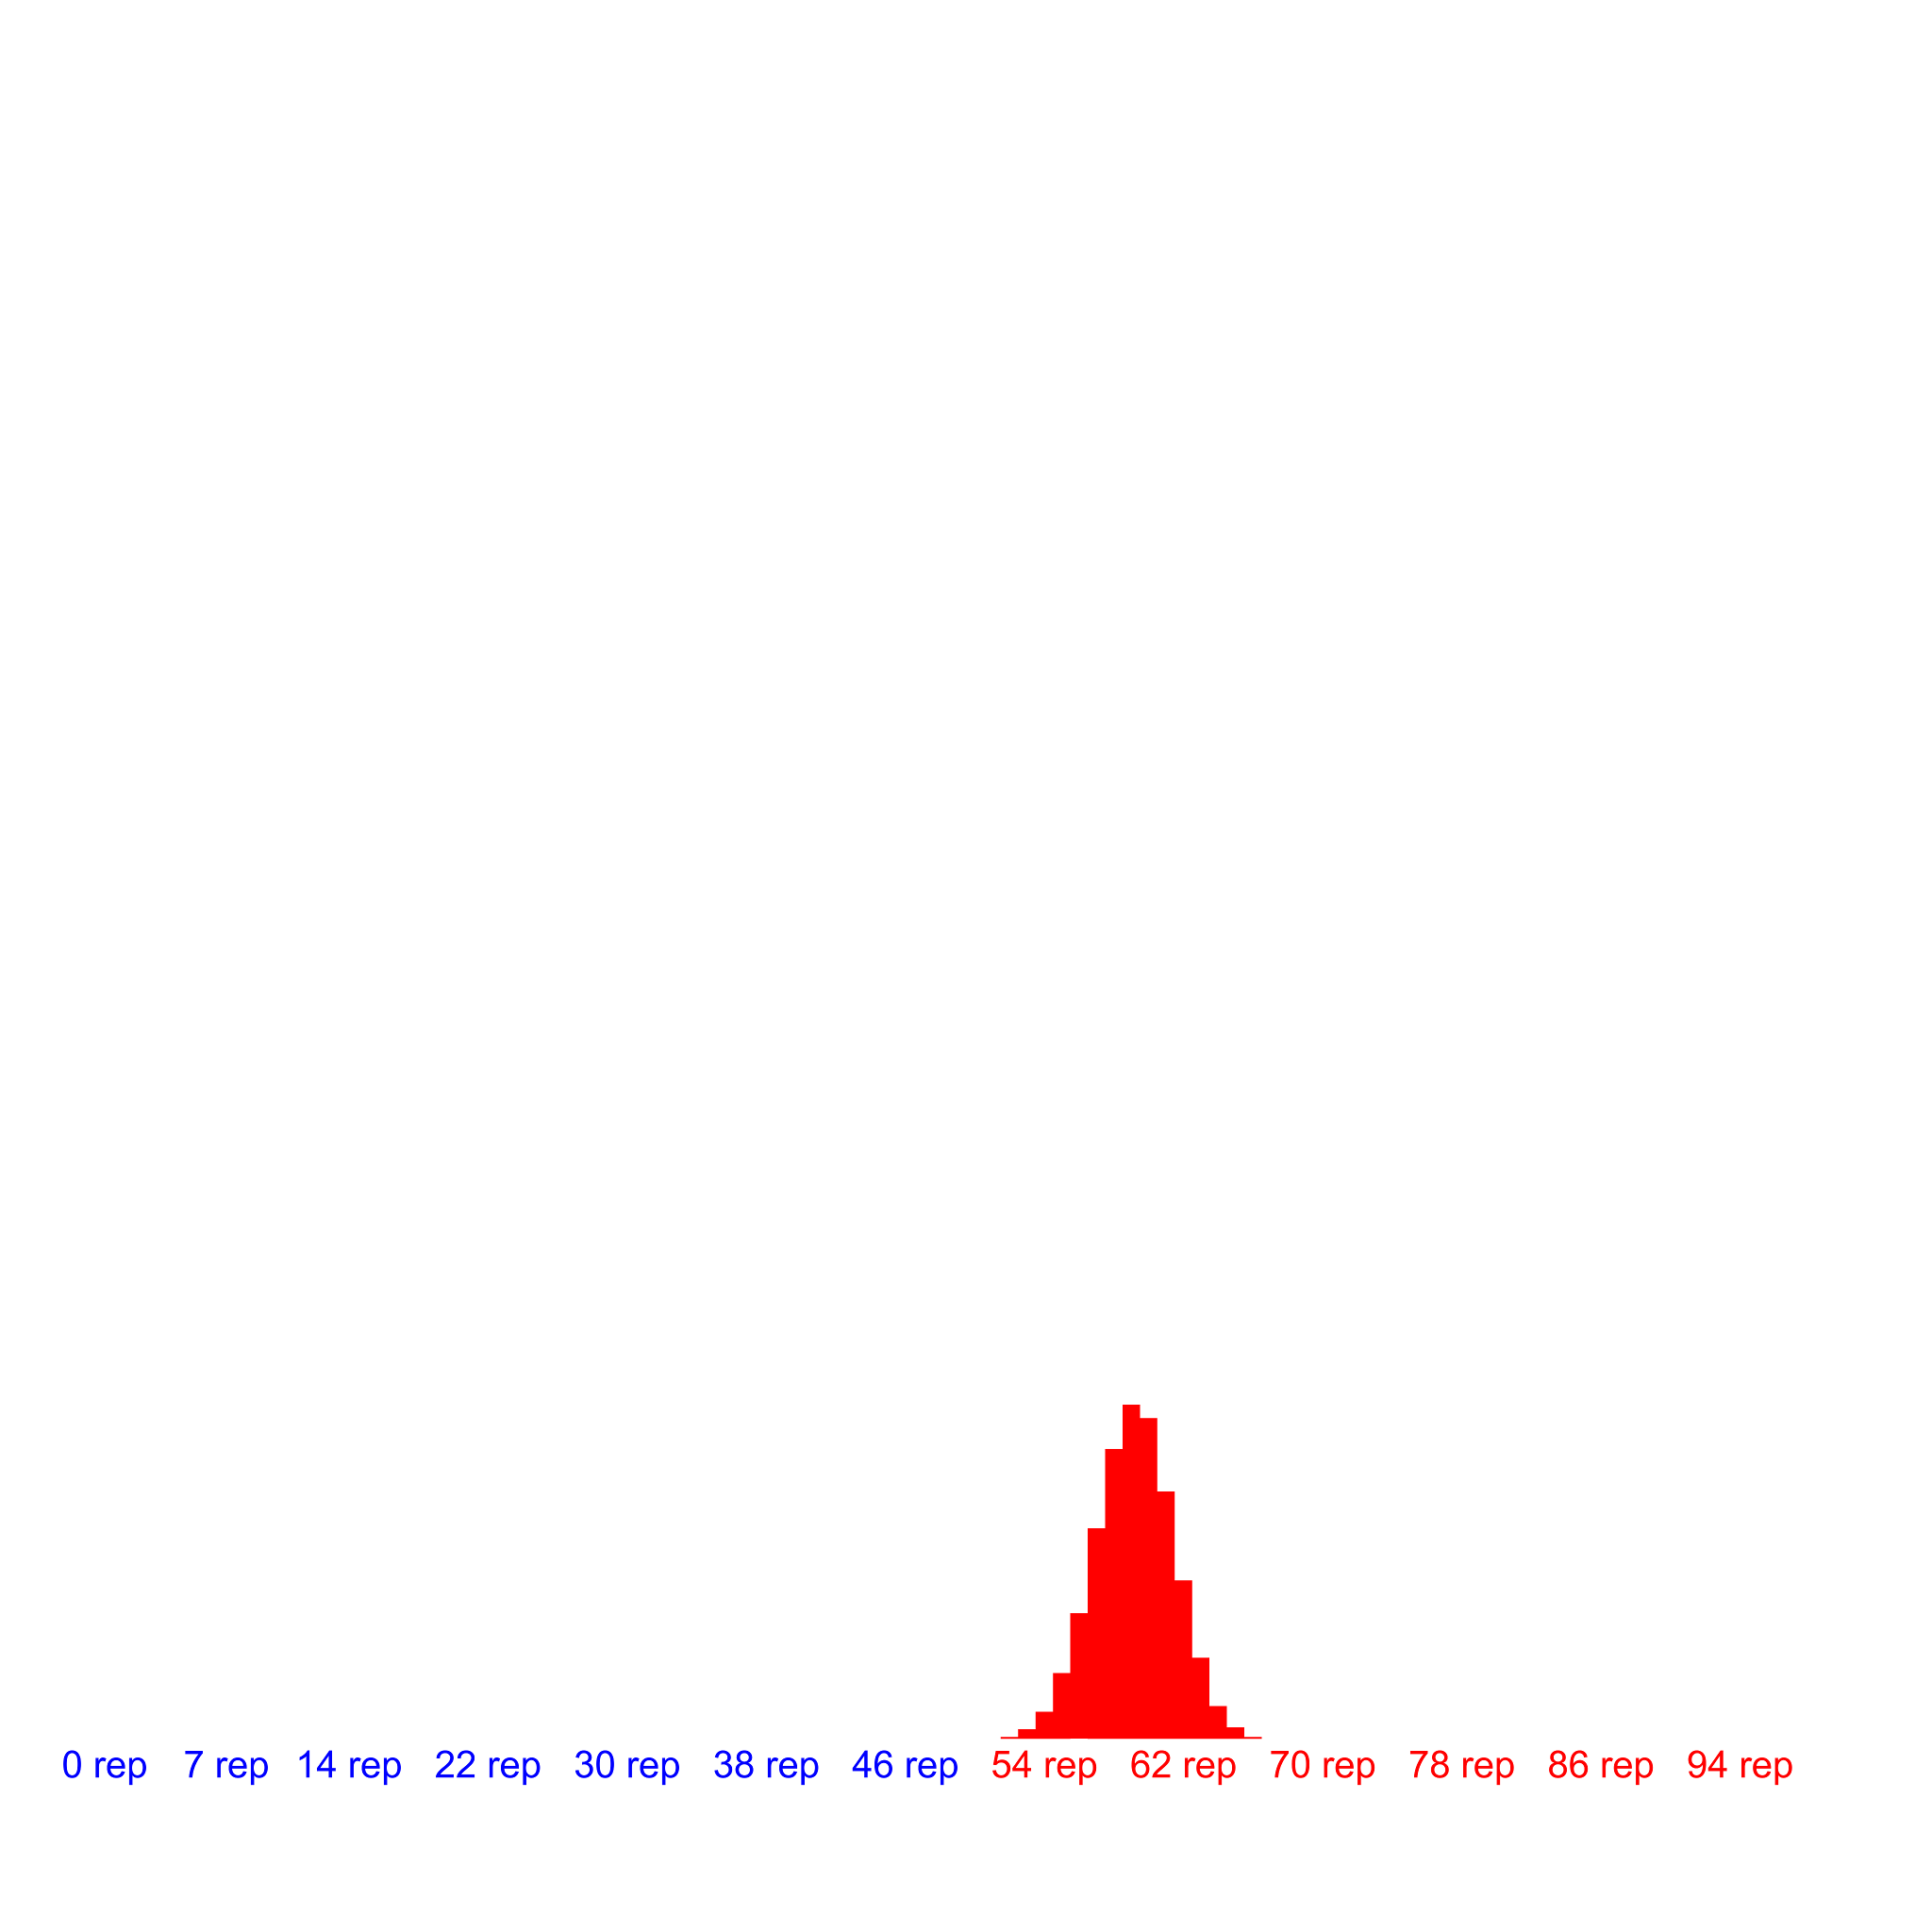
\includegraphics[scale=0.25]{../Figures/WI2010/seats.png}
        \caption{Seat count likelihoods generated from the probability model for Wisconsin 2010 Assembly districts}\label{fig:LikelihoodsSeatCounts}
    \end{center}
\end{figure}
 

\subsubsection{Specific partisan asymmetry likelihoods}
 
To get the likelihood function for partisan asymmetry, we again use Monte-Carlo numerical integration, but this time we subtract the seat counts Democrats would get with that share of the vote from the number Republicans would get under the same share of the vote. The results are shown in figure \ref{fig:LikelihoodsAsymmetry}.
 
\begin{figure}[htb!]
    \begin{center}
        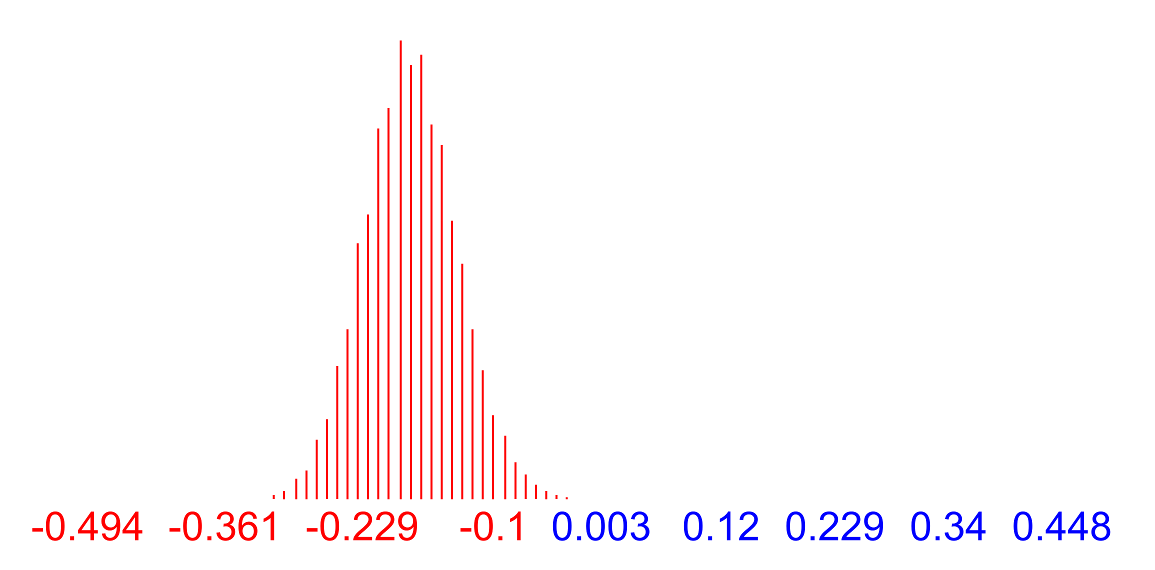
\includegraphics[scale=0.5]{../Figures/WI2010/asymmetry_alt.png}
        \caption{Specific asymmetry likelihoods generated from the probability model for Wisconsin 2010 Assembly districts}\label{fig:LikelihoodsAsymmetry}
    \end{center}
\end{figure}
 
Note the mode of the distribution - the most likely result - is a partisan asymmetry of 20\% of the available seats.  For instance, the most likely result might be that Republicans get 6/10ths of the legislative seats, whereas if the popular vote count were reversed, Democrats would get only 4/10th of the legislative seats.  Remedying this would give Democrats 10\% more seats.  This means that roughly 10\% of the entire Democratic-voting population of the state of Wisconsin were effectively disenfranchised, in violation of the one person, one vote principle.  Conversely, 10\% of the Republican-voting population effectively got an extra vote.  That's approximately 306,000 felonies.
 
Note, out of 100,000 sample points, none of them resulted in specific partisan asymmetry favoring Democrats.  Since an assembly district election occurs every 2 years, this shows that, without significant changes in geo-spatial demographics, the asymmetric pro-Republican partisan advantage inherent in this redistricting will persist for the next 200,000 years.  (Though no doubt there will be significant geo-spatial demographic changes before then.  Indeed, there will probably even be some geological changes.)

\subsection{Discussion of results}
\subsubsection{The effect of the gerrymandering is extreme, and durably so.}
 
Taken together, the descriptive statistics (mode, expectation, dispersion, likelihood of crossing zero, etc.) for the specific partisan asymmetry likelihood function for the 2010-census cycle Wisconsin assembly districts, show both an extreme level of partisan gerrymandering with very real and quantifiable harm to the citizens, and that this partisan asymmetry is very durable; that it will almost certainly continue to cause harm, and likely at an extreme level.
 
\subsubsection{The hyper-partisan nature of Wisconsin state legislature amplifies disenfranchisement caused by gerrymandering, effectively disenfranchising ALL voters.}
 
The congressional record provides ample evidence that -- like many congresses in the United States -- most votes in the Wisconsin assembly are party-line.  Consequently, the party that holds the congressional majority has full control, and the minority party has none, with the exception of being able to block legislation with a filibuster, if and only if they have at least 1/3 of the seats.
 
Without the present gerrymander, congressional majority power would be up for grabs, and subject to the will and review of the voting populace, with about a 50\% chance for either party to have it.  Congressional power would be both determined by the voters, and accountable to them.
 
With the present gerrymander, it is neither.  Republican control is both absolute and durable.  Democrats' only hope of blocking Republican legislation is a filibuster, which they have only about a 50\% chance of having the numbers for.  Their chance of passing any meaningful legislation is practically nil, since even in the most extreme swings in voter sentiment, Republicans will still hold a sizable congressional majority.
 
When it comes to what legislation gets passed or does not get passed, despite fully half of the state population having Democratic political beliefs, effectively none of them are represented, both now, and in the foreseeable future.  
 
\subsubsection{If this harm is not remedied by 2020, Republicans will be in a position to renew it for another decade.}
 
As our analysis shows, with over 99.99\% certainty, come the next redistricting cycle in 2020, Republicans will still hold a majority in the state legislature, regardless of how the sentiments of voters have changed in the interim.  With the redistricting power that comes with that, they will be able to repeat the same foul play they did in 2010, thus guaranteeing them control of the state legislature, and immunity from the democratic voice of ALL citizens of Wisconsin, for an additional decade. In other words, the systematic disenfranchisement of Wisconsin voters perpetrated by the state legislature in 2010 has put that same legislature in a position to continue to disenfranchise voters through the 2020 redistricting cycle. Since state legislatures control the redistricting process, gerrymandered legislative maps not only confer an ill gotten partisan advantage, but they shield those perpetrating the gerrymander from accountability at the ballot box. Therefore, without a judicial remedy protecting the rights of voters from legislatures seeking to disenfranchise them, it is likely that extreme partisan bias will become a permanent feature in the Wisconsin state legislative maps.



\section{Conclusions}

\subsection{Can be combined with any existing test to give more information}
 
The method we've outlined consists of two parts: 
Computing future election result likelihood distributions from historical data
Numerically integrating those distributions to get likelihood functions for specific measures or tests
 
In this paper we used three different measures for the second part:
District partisanship histogram,
Statewide seat count likelihoods, and 
Specific partisan asymmetry likelihoods
 
It is important to note that any measure or test can be used in the second part.  Whether it's Sam Wang's median minus mean (Wang 2016), Grofman and King's partisan asymmetry  (Grofman and King 2007), the geometric area of partisan asymmetry described by Nagle (Nagle 2015), the measure supplied in this paper, "specific partisan asymmetry", or even measures of totally different properties such as competitiveness or voting power.
 
In other words, this method can be combined with any current or future measure or test to augment that measure, thus making it provide more information.
 
\subsection{Enables measuring robustness / durability}
 
When a measure is combined with the first part in this way, what once was a single statistic on a single, past election, becomes an entire likelihood distribution of all possible election outcomes, past, present, and future.
 
Consequently, this method, when added to any other method or test, extends that method or test to show durability.  This allows one to distinguish between results due to chance fluctuations, and results that are systemic and durable features of the partisan distribution of voters among the districts.


\clearpage
\section*{}
%\bibliographystyle{plainnat}
%\bibliography{Hyperelas,Bib2}
\clearpage



\end{document}
